% begin module trig-example
\begin{frame}
\begin{example}
\begin{columns}[c]
\column{.5\textwidth}

\psset{xunit=1.8cm,yunit=1.8cm}
\begin{pspicture}(-2.3,-0.5)(0.5,2.2)
\psframe*[linecolor=white, fillcolor=white](-2.3,-0.5)(0.8,2.5)
\psaxes[fillcolor=white, fillstyle=solid, labels=none, ticks=none]{<->}(0,0)(-2.3,-0.5)(0.5,2.2)
\rput[l](0.55, 0){$x$}
\rput[b](0, 2.25){$y$}

\psline[linecolor=blue](0,0)(-1,1.732)
\psline[linecolor=blue](0,0)(0.5,0)
\uncover<3->{
\psline[linestyle=dotted](-1,1.732)(-1, 0)
\psline[linestyle=dotted](-1,1.732)(0, 1.732)
}
\pscircle*(-1,1.732){0.07}

\rput[l](0.15, 0.35){$\frac{2\pi}{3}$}
\psarc[linecolor=red](0,0){0.5}{0}{120}
\uncover<2->{
\rput(-0.25, 0.15){$\frac{\pi}{3}$}
\psarc[linecolor=red](0,0){0.3}{120}{180}
}
\uncover<3->{
\rput[br](-1,1.732){$(-1,\sqrt{3})$}
\alert<5,7,11,13>{\rput[lb](-0.45, 0.85){$2$}}
\alert<5,9,11,15>{\rput[r](-1.1, 0.85){$\sqrt{3}$}}
\rput[t](-1, -0.05){$(\alert<7,9,13,15>{-1},0)$}
}
\end{pspicture}
%\ \only<handout:0| -1>{%
%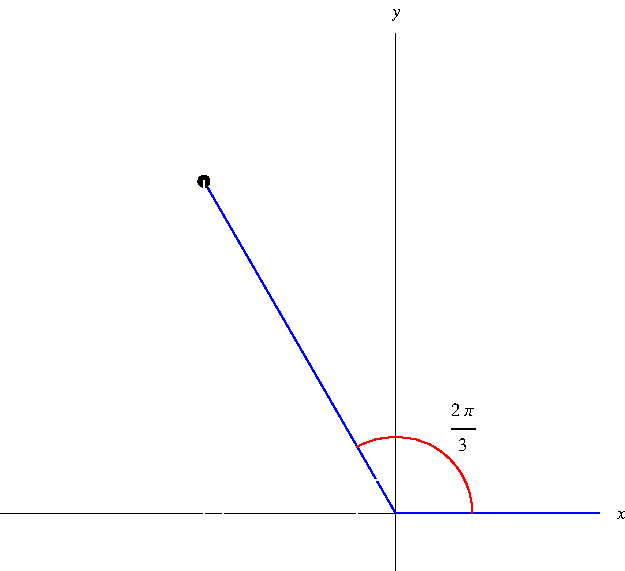
\includegraphics[width=5cm]{trigonometry/pictures/app-d-ex3a.pdf}%%
%}%
%\only<handout:0| 2>{%
%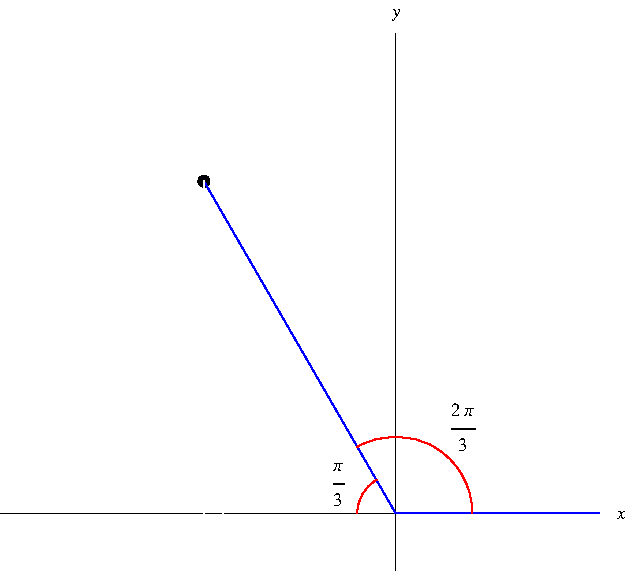
\includegraphics[width=5cm]{trigonometry/pictures/app-d-ex3b.pdf}%%
%}%
%\only<3->{%
%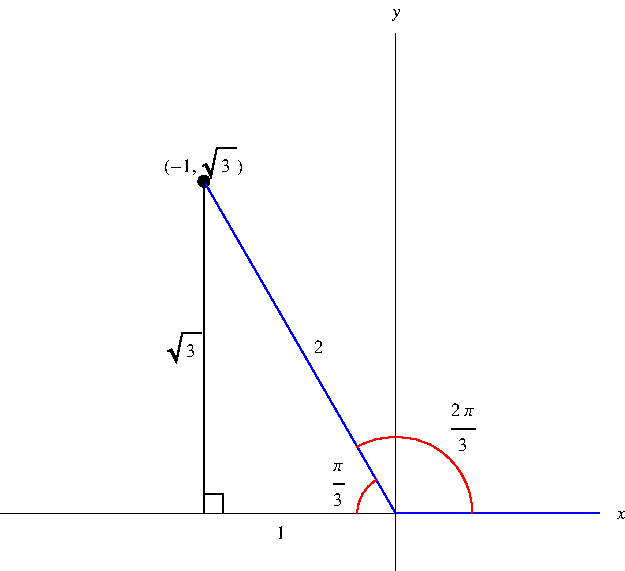
\includegraphics[width=5cm]{trigonometry/pictures/app-d-ex3c.pdf}%%
%}%
\column{.5\textwidth}
Find the exact trigonometric ratios for $\theta = 2\pi /3=120^\circ$.
\end{columns}
\begin{align*}
\alert<handout:0| 4-5>{\sin \frac{2\pi}{3}} & \alert<handout:0| 4-5>{= \uncover<5->{\frac{\sqrt{3}}{2}}} &
\alert<handout:0| 6-7>{\cos \frac{2\pi}{3}} & \alert<handout:0| 6-7>{= \uncover<7->{-\frac{1}{2}}} &
\alert<handout:0| 8-9>{\tan \frac{2\pi}{3}} & \alert<handout:0| 8-9>{= \uncover<9->{\frac{\sqrt{3}}{-1}= -\sqrt{3}}} \\
\alert<handout:0| 10-11>{\csc \frac{2\pi}{3}} & \alert<handout:0| 10-11>{= \uncover<11->{\frac{2}{\sqrt{3}}}} &
\alert<handout:0| 12-13>{\sec \frac{2\pi}{3}} & \alert<handout:0| 12-13>{= \uncover<13->{-\frac{2}{1}=-2}} &
\alert<handout:0| 14-15>{\cot \frac{2\pi}{3}} & \alert<handout:0| 14-15>{= \uncover<15->{-\frac{1}{\sqrt{3}}}}
\end{align*}
\end{example}
\end{frame}
% end module trig-example